\documentclass[tikz,border=5pt]{standalone}
\usepackage{tikz}
\usepackage{graphicx}
\pagestyle{empty}
\begin{document}
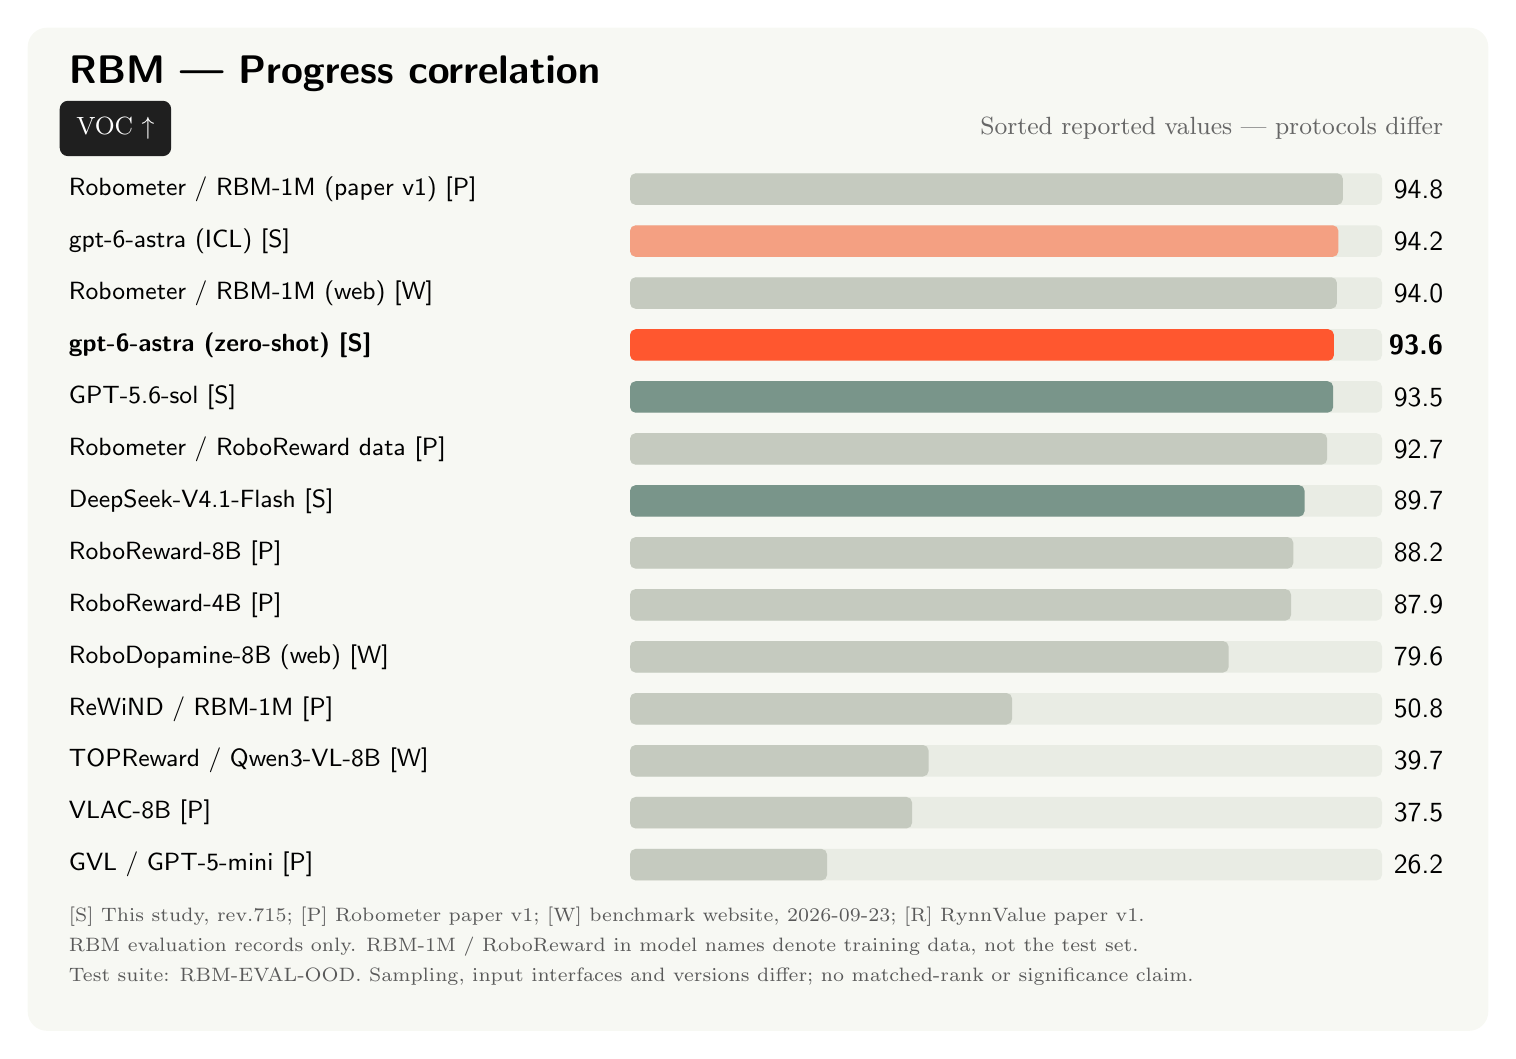
\begin{tikzpicture}[x=1cm,y=1cm,font=\sffamily]
\definecolor{cardbg}{HTML}{F7F8F3}
\definecolor{trackbg}{HTML}{E9ECE4}
\definecolor{mutedbar}{HTML}{C5CABF}
\definecolor{astrabar}{HTML}{FF572F}
\definecolor{iclbar}{HTML}{F4A082}
\definecolor{studybar}{HTML}{79958A}
\fill[cardbg,rounded corners=7pt] (-.4,1.8) rectangle (18.15,-10.94);
\node[anchor=west,font=\sffamily\bfseries\Large] at (0,1.22) {RBM | Progress correlation};
\node[anchor=west,fill=black!88,text=white,rounded corners=3pt,inner sep=6pt,font=\small] at (0,.52) {VOC $\uparrow$};
\node[anchor=east,text=black!60,font=\small] at (17.7,.52) {Sorted reported values | protocols differ};
\node[anchor=west,font=\sffamily\small] at (0,-0.25) {Robometer / RBM-1M (paper v1) [P]};
\fill[trackbg,rounded corners=2pt] (7.25,-0.45) rectangle (16.8,-0.05);
\fill[mutedbar,rounded corners=2pt] (7.25,-0.45) rectangle (16.303400,-0.05);
\node[anchor=east,font=\sffamily] at (17.7,-0.25) {94.8};
\node[anchor=west,font=\sffamily\small] at (0,-0.91) {gpt-6-astra (ICL) [S]};
\fill[trackbg,rounded corners=2pt] (7.25,-1.11) rectangle (16.8,-0.71);
\fill[iclbar,rounded corners=2pt] (7.25,-1.11) rectangle (16.246100,-0.71);
\node[anchor=east,font=\sffamily] at (17.7,-0.91) {94.2};
\node[anchor=west,font=\sffamily\small] at (0,-1.57) {Robometer / RBM-1M (web) [W]};
\fill[trackbg,rounded corners=2pt] (7.25,-1.77) rectangle (16.8,-1.37);
\fill[mutedbar,rounded corners=2pt] (7.25,-1.77) rectangle (16.227000,-1.37);
\node[anchor=east,font=\sffamily] at (17.7,-1.57) {94.0};
\node[anchor=west,font=\sffamily\small\bfseries] at (0,-2.23) {gpt-6-astra (zero-shot) [S]};
\fill[trackbg,rounded corners=2pt] (7.25,-2.43) rectangle (16.8,-2.03);
\fill[astrabar,rounded corners=2pt] (7.25,-2.43) rectangle (16.188800,-2.03);
\node[anchor=east,font=\sffamily\bfseries] at (17.7,-2.23) {93.6};
\node[anchor=west,font=\sffamily\small] at (0,-2.89) {GPT-5.6-sol [S]};
\fill[trackbg,rounded corners=2pt] (7.25,-3.09) rectangle (16.8,-2.69);
\fill[studybar,rounded corners=2pt] (7.25,-3.09) rectangle (16.179250,-2.69);
\node[anchor=east,font=\sffamily] at (17.7,-2.89) {93.5};
\node[anchor=west,font=\sffamily\small] at (0,-3.55) {Robometer / RoboReward data [P]};
\fill[trackbg,rounded corners=2pt] (7.25,-3.75) rectangle (16.8,-3.35);
\fill[mutedbar,rounded corners=2pt] (7.25,-3.75) rectangle (16.102850,-3.35);
\node[anchor=east,font=\sffamily] at (17.7,-3.55) {92.7};
\node[anchor=west,font=\sffamily\small] at (0,-4.21) {DeepSeek-V4.1-Flash [S]};
\fill[trackbg,rounded corners=2pt] (7.25,-4.41) rectangle (16.8,-4.01);
\fill[studybar,rounded corners=2pt] (7.25,-4.41) rectangle (15.816350,-4.01);
\node[anchor=east,font=\sffamily] at (17.7,-4.21) {89.7};
\node[anchor=west,font=\sffamily\small] at (0,-4.87) {RoboReward-8B [P]};
\fill[trackbg,rounded corners=2pt] (7.25,-5.07) rectangle (16.8,-4.67);
\fill[mutedbar,rounded corners=2pt] (7.25,-5.07) rectangle (15.673100,-4.67);
\node[anchor=east,font=\sffamily] at (17.7,-4.87) {88.2};
\node[anchor=west,font=\sffamily\small] at (0,-5.53) {RoboReward-4B [P]};
\fill[trackbg,rounded corners=2pt] (7.25,-5.73) rectangle (16.8,-5.33);
\fill[mutedbar,rounded corners=2pt] (7.25,-5.73) rectangle (15.644450,-5.33);
\node[anchor=east,font=\sffamily] at (17.7,-5.53) {87.9};
\node[anchor=west,font=\sffamily\small] at (0,-6.19) {RoboDopamine-8B (web) [W]};
\fill[trackbg,rounded corners=2pt] (7.25,-6.39) rectangle (16.8,-5.99);
\fill[mutedbar,rounded corners=2pt] (7.25,-6.39) rectangle (14.851800,-5.99);
\node[anchor=east,font=\sffamily] at (17.7,-6.19) {79.6};
\node[anchor=west,font=\sffamily\small] at (0,-6.85) {ReWiND / RBM-1M [P]};
\fill[trackbg,rounded corners=2pt] (7.25,-7.05) rectangle (16.8,-6.65);
\fill[mutedbar,rounded corners=2pt] (7.25,-7.05) rectangle (12.101400,-6.65);
\node[anchor=east,font=\sffamily] at (17.7,-6.85) {50.8};
\node[anchor=west,font=\sffamily\small] at (0,-7.51) {TOPReward / Qwen3-VL-8B [W]};
\fill[trackbg,rounded corners=2pt] (7.25,-7.71) rectangle (16.8,-7.31);
\fill[mutedbar,rounded corners=2pt] (7.25,-7.71) rectangle (11.041350,-7.31);
\node[anchor=east,font=\sffamily] at (17.7,-7.51) {39.7};
\node[anchor=west,font=\sffamily\small] at (0,-8.17) {VLAC-8B [P]};
\fill[trackbg,rounded corners=2pt] (7.25,-8.37) rectangle (16.8,-7.97);
\fill[mutedbar,rounded corners=2pt] (7.25,-8.37) rectangle (10.831250,-7.97);
\node[anchor=east,font=\sffamily] at (17.7,-8.17) {37.5};
\node[anchor=west,font=\sffamily\small] at (0,-8.83) {GVL / GPT-5-mini [P]};
\fill[trackbg,rounded corners=2pt] (7.25,-9.03) rectangle (16.8,-8.63);
\fill[mutedbar,rounded corners=2pt] (7.25,-9.03) rectangle (9.752100,-8.63);
\node[anchor=east,font=\sffamily] at (17.7,-8.83) {26.2};
\node[anchor=west,text=black!65,font=\scriptsize] at (0,-9.49) {[S] This study, rev.715; [P] Robometer paper v1; [W] benchmark website, 2026-09-23; [R] RynnValue paper v1.};
\node[anchor=west,text=black!65,font=\scriptsize] at (0,-9.87) {RBM evaluation records only. RBM-1M / RoboReward in model names denote training data, not the test set.};
\node[anchor=west,text=black!65,font=\scriptsize] at (0,-10.25) {Test suite: RBM-EVAL-OOD. Sampling, input interfaces and versions differ; no matched-rank or significance claim.};
\end{tikzpicture}
\end{document}
